%TODO zweryfikować ten dokument jak już zaktualizują ubuntu.com
%obrazek
%linki
%rozmiar obrazów instalacyjnych
\begin{wrapfigure}{L}{0.6\textwidth}
	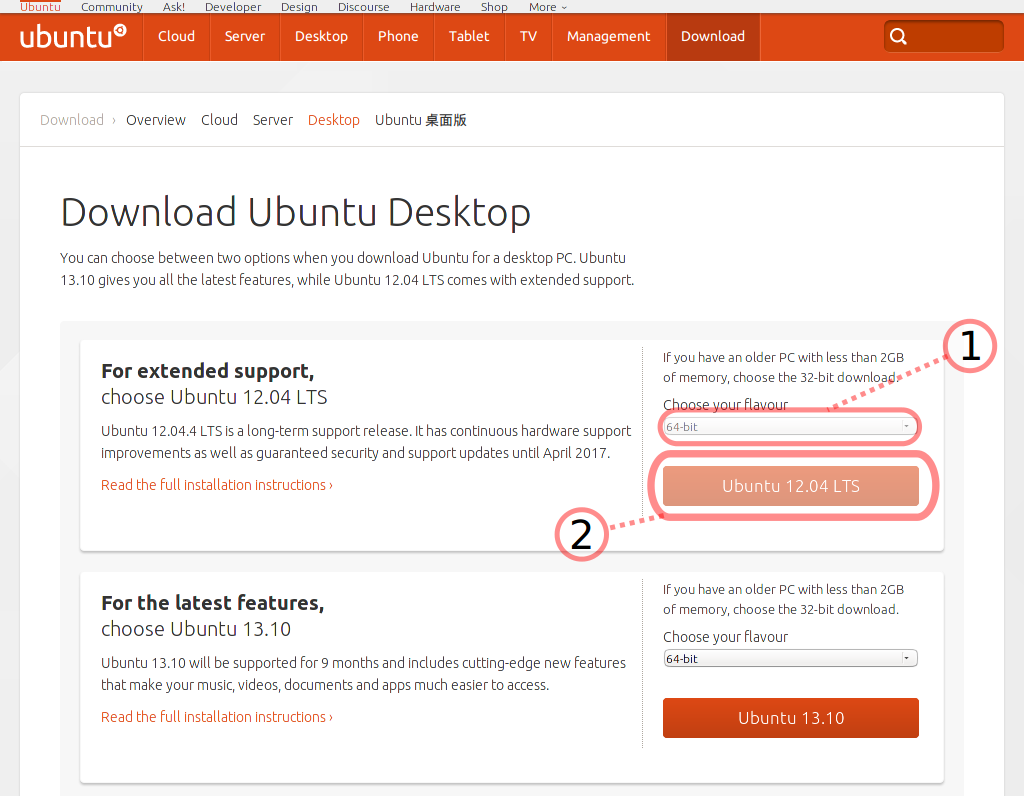
\includegraphics[scale=0.45]{images/instalacja_pobieranie_obrazu.png}
\end{wrapfigure}
Pierwszym etapem instalacji systemu jest pobranie instalatora. W tym celu udaj się na stronę \href{http://www.ubuntu.com/download/desktop}{ubuntu.com} i z górnego paska wybież \textcolor{ubuntu_orange}{Download} a następnie \textcolor{ubuntu_orange}{Desktop}
\begin{description}
\item[(1) Wybór wersji systemu]To pole pozwali ci wybrać pomiędzy 32 a 64 bitową wersją systemu. Domyślnie wybrana jest opcja 64 bitowa. 
\item[(2)]Kliknij na ten przycisk aby przejśc do kolejnego ekranu.
\end{description}
Na kolejnym ekranie będziesz mieć możliwość przekazania dotacji na rzecz Ubuntu. W tym momencie nas to nie interesuje. Przesuń stronę w dół i kliknij na \textcolor{ubuntu_orange}{Not now, take me to the download}. Zostaniesz przeniesiony na kolejną stronę, pobieranie obrazu systemu rozpocznie się za kilka sekund.

Jeżeli twój komputer został wyprodukowany nie dawnej niż 5 lat temu, wersja 64 bitowa będzie na pewno odpowiednia. Jeżeli masz mniej niż 2 gigabajty RAMu, wybierz wersję 32 bitową. Niezależnie jaką wersję wybierzesz, bedziesz mieć dostęp do takiego samego zestawu oprogramowania. Wersja 64 bitowa jest lepiej dopasowana do nowoczesnych systemów. Jeżeli masz jakiekolwiek wątpliwości to wybierz wersję 32 bitową. Taka wersja systemu będzie działać także na 64 bitowym komputerze. Po prostu nie będzie wykorzystywać wszystkich jego możliwości.

Linki do pobierania bezpośredniego:
\begin{itemize}
\item \href{http://www.ubuntu.com/start-download?distro=desktop&bits=64&release=lts}{Wersja 64 bitowa (733 megabajtów).}
\item \href{http://www.ubuntu.com/start-download?distro=desktop&bits=32&release=lts}{Wersja 32 bitowa (731 megabajtów).}
\end{itemize}
\clearpage